\graphicspath{chapters/latency/img/}

\section{Latency over whole Data Range} \label{sec:latency-wholerange}

The performance of Starlink latency has changed over time. We looked at RIPE Atlas TLS data that has been collected by built-in measurements (i.e., measurements that are continuously running in each individual probe in a fixed time interval).

\begin{figure}
	\centering
	\begin{subfigure}[b]{0.4\textwidth}
		\centering
		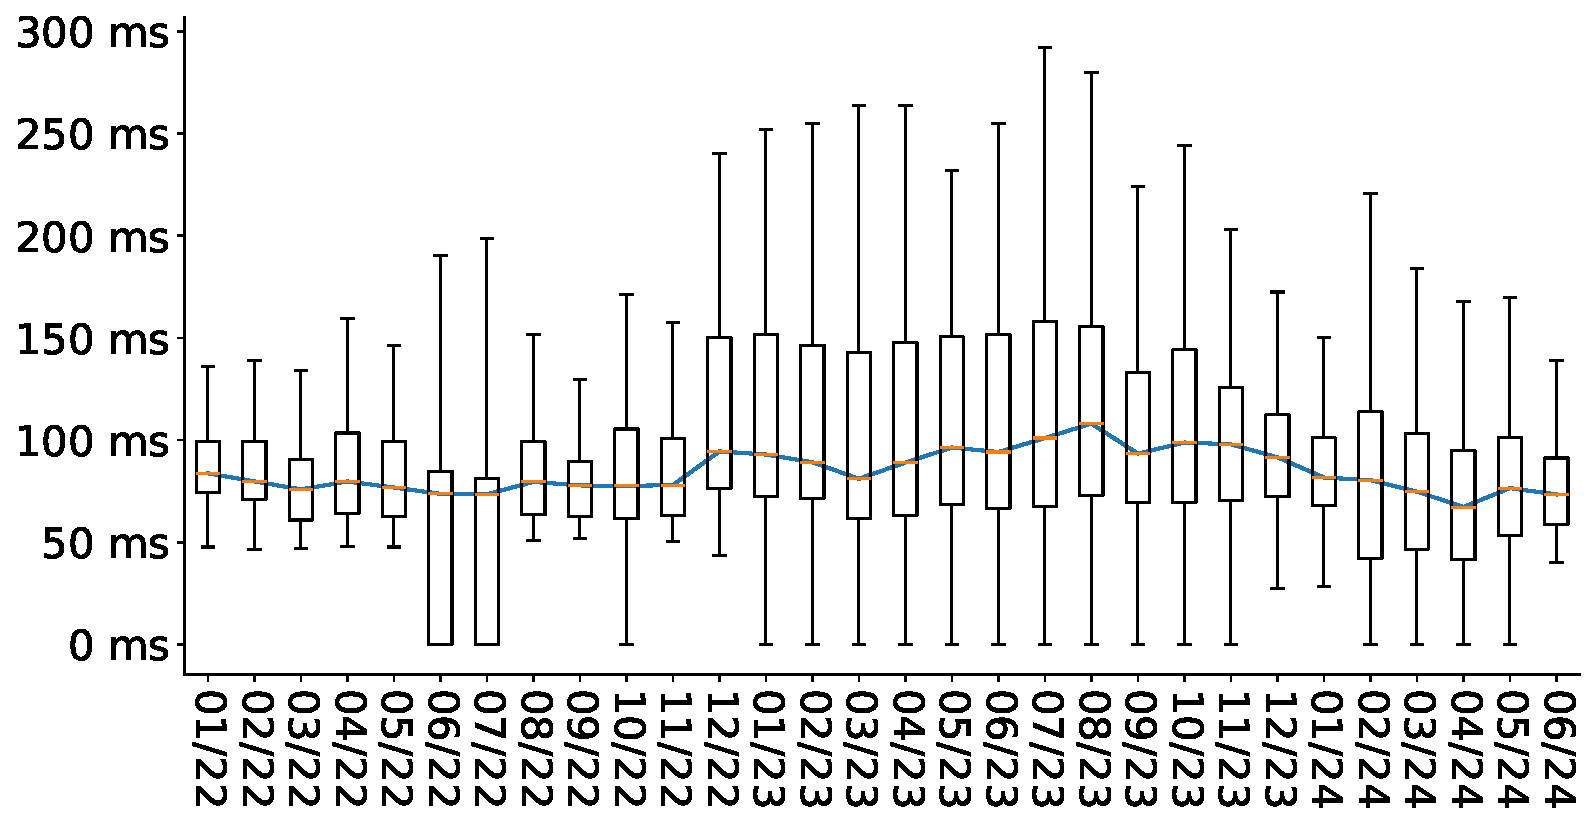
\includegraphics{latency_2022_to_2024_Germany.pdf}
	\end{subfigure}
	\hfill
	\begin{subfigure}[b]{0.4\textwidth}
		\centering
		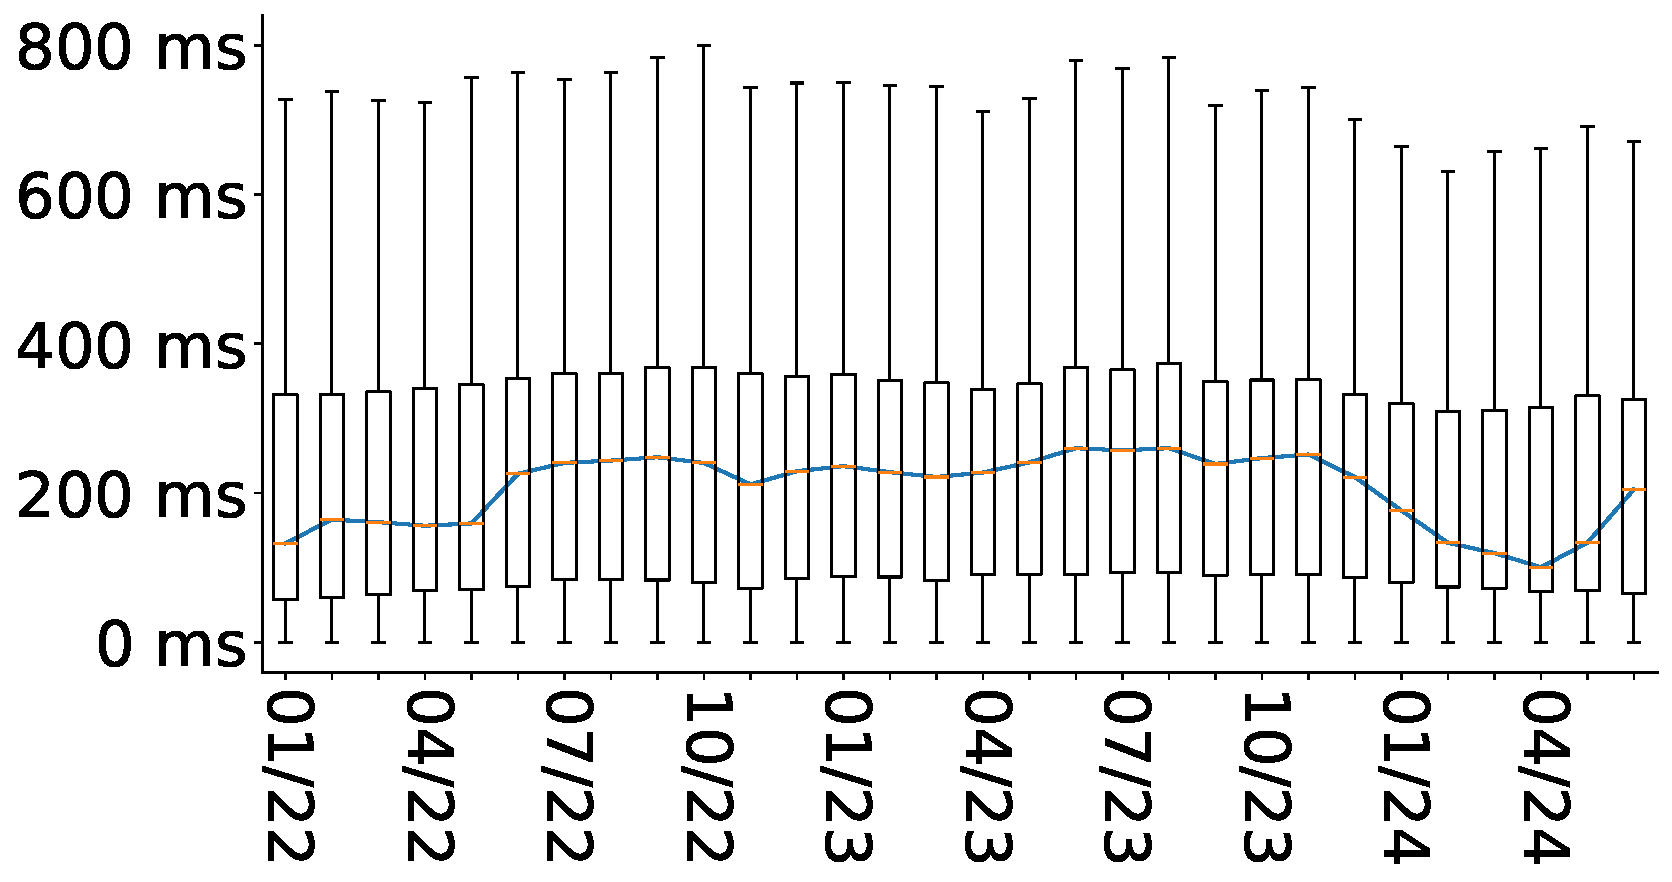
\includegraphics{latency_2022_to_2024_United States.pdf}
	\end{subfigure}
	\hfill
	\begin{subfigure}[b]{0.4\textwidth}
		\centering
		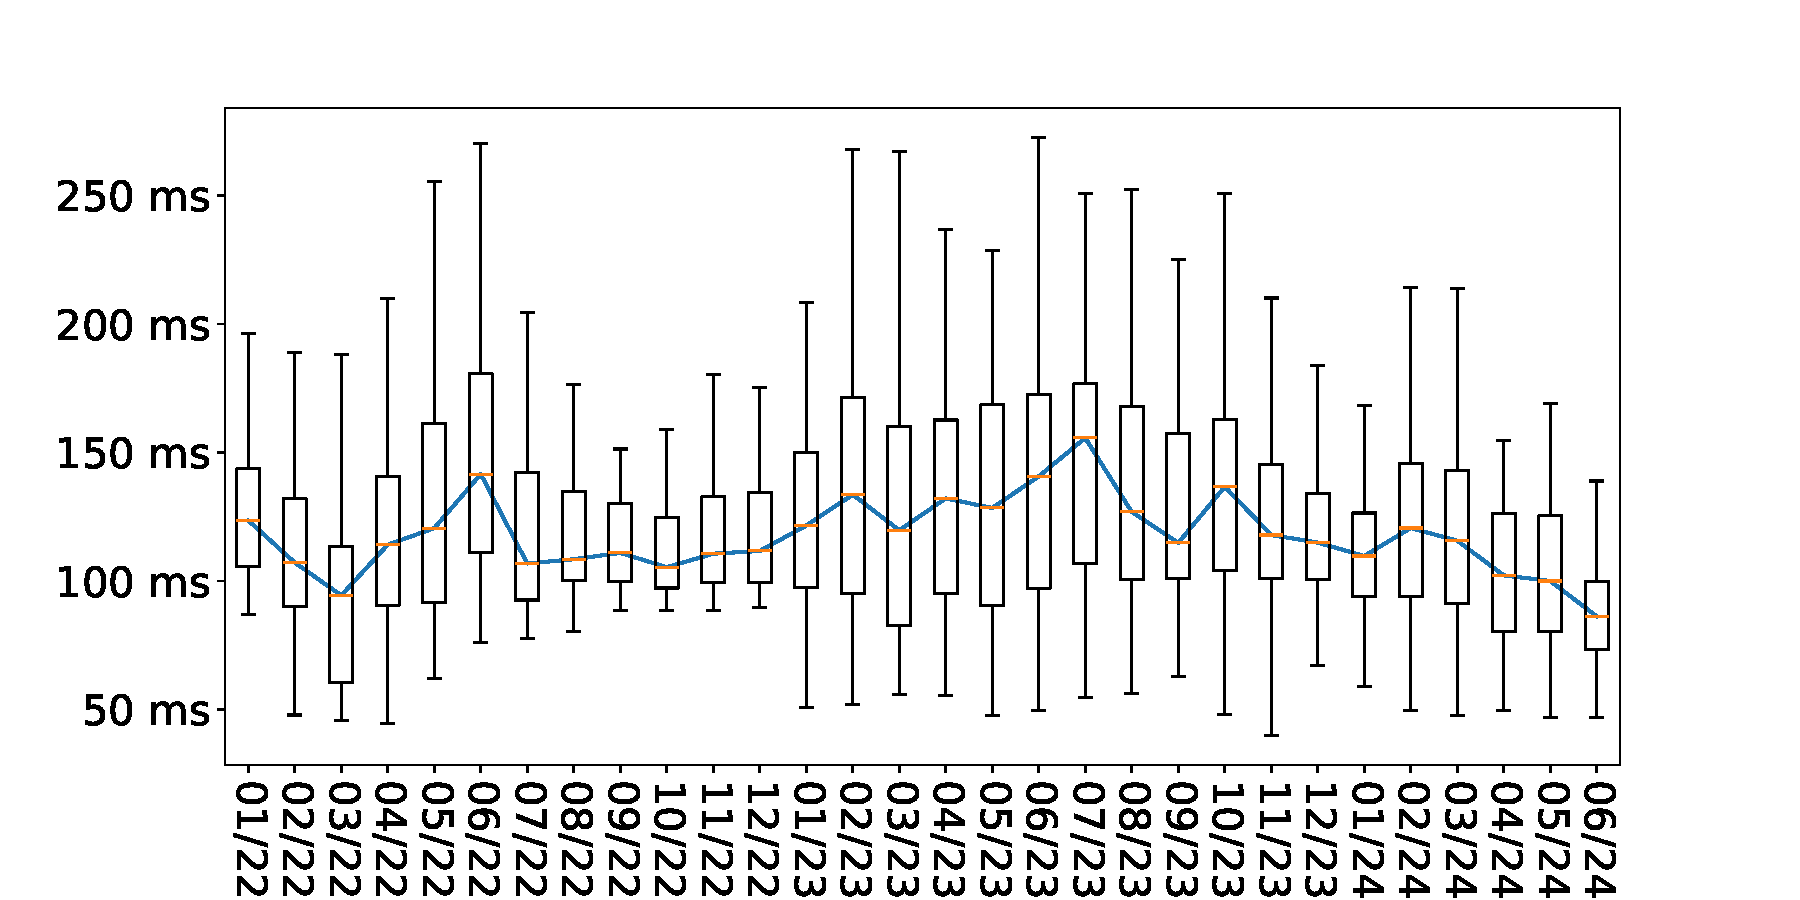
\includegraphics{latency_2022_to_2024_Poland.pdf}
	\end{subfigure}
	\hfill
	\begin{subfigure}[b]{0.4\textwidth}
		\centering
		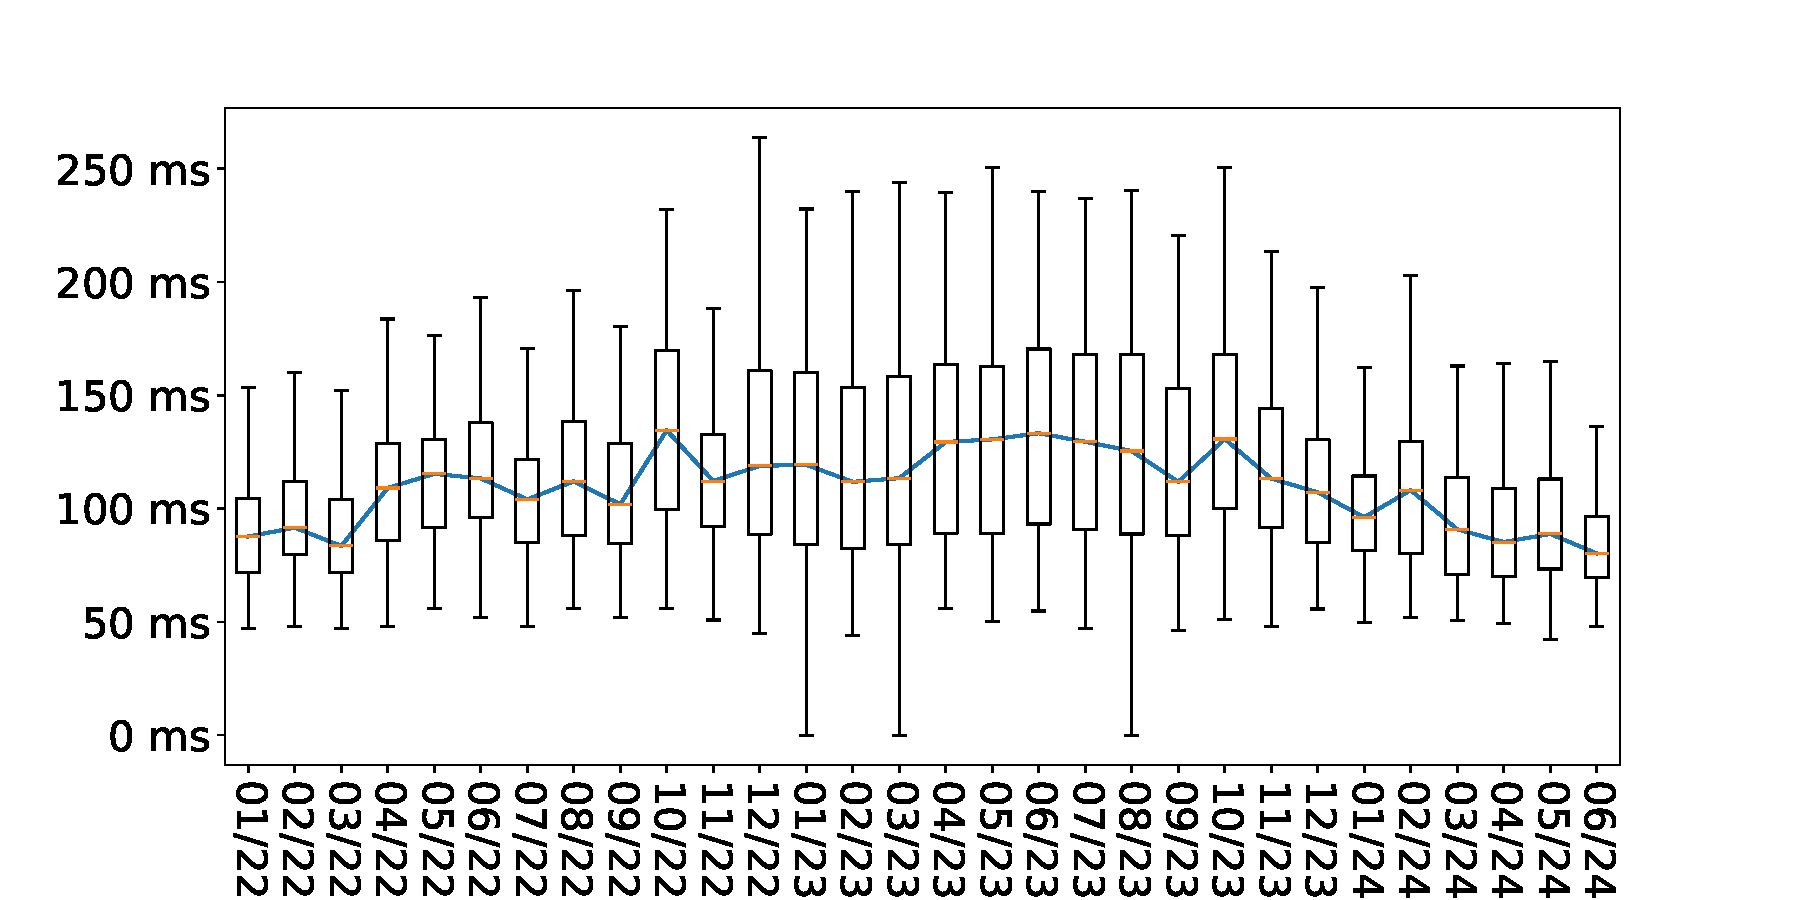
\includegraphics{latency_2022_to_2024_Austria.pdf}
	\end{subfigure}
	\label{fig:latency-wholerange}
	\caption{Latency History for Germany, the USA, Poland, and Austria in the period 01/2022 to 06/2024}
\end{figure}

Figure~\ref{fig:latency-wholerange} shows the history of median latencies from January~2022 until June~2024 for Germany, the United States, Poland, and Austria\footnote{These countries were chosen due to the completeness of data}.

One can see that the median latency is usually at around 100 to 150~ms for most countries. However, in 2022 the latency was lower compared to 2023. Most of the countries observed show an upwards trend in the late months of 2022 (most of the time in December). In the late months of 2023, the latency starts to decline again. In the last couple of months, we observe an increase in latency once again.

We assume the reason for a rise of latency in the congestion of the Starlink network. In the recent time Starlink extended their availability across more countries allowing more users, especially those in countries with less networking infrastructure, to access the network.
On the contrary, Starlink also launched more satellites (2022: 3481, 2024: 5700+) and added more \ac{PoP} which likely reduces the congestion.

However, countries still vary a lot in performance. This is due to various different factors, e.g., weather, ground station infrastructure,
